% !TeX root = ../../../book.tex
\section{计数论证}

现在,我们已经完全准备好解决本章的主要问题了!我们将运用之前介绍的计数技术——乘法原理和加法原理——以及选择与排列的公式。更重要的是,我们将展示一些标准的计数论证和证明策略。在此过程中,我们会指出通用的指导原则和证明方法,并通过若干示例来解释和应用这些技术。这些都是我们希望你在未来能够掌握并应用的方法。

% !TeX root = ../../../book.tex

\subsection{扑克牌型}

\begin{example}[一对]

    让我们从最简单的情况开始,计算一下一对牌型的数量。我们要强调的是,这里只计算正好是一对的牌型,不包含两对、三条、葫芦和四条。这一思路将在我们接下来的计数过程中逐步展现。(这也提示了为什么计算``高牌''牌型实际上非常复杂,比仅仅选择五张随机牌要难得多!我们如何保证一手牌没有重复的牌,不是顺子,也不是同花?我们将在本节后面讨论这个问题。)

    在这个例子中 --- 以及我们将要解释的每个其他例子中,还有你将完成的每个练习中(你感觉到这很重要吗?) --- 我们将寻找一种方法,通过这种方法我们能构建出具有特定属性的对象(在这种情况下,是一手正好有一对且不是其他牌型的扑克牌)。通过计算每一步的选择数量,并确保每个期望的对象只能通过一种选择组合得到,我们可以应用乘法法则,确定具有期望属性的对象数量。

    这里有一个有用的策略来设计这种方法:假设你的朋友手里拿着你要计算的一个对象,但你看不到它。你会问什么问题来确定他/她手中对象的特定属性?这些问题可以是是/否问题,或者更常见的是关于对象特定属性的询问。在我们的具体情况下,计算一对牌型,我们可能会问以下问题:
    \begin{enumerate}[label=(\arabic*)]
        \item ``一对中的两张牌是什么?''
        \item ``不在一对中的三张牌是什么?''
    \end{enumerate}
    通过这些问题的答案,我们可以完全确定朋友手中的牌。不幸的是,直接这样问,计算这些问题的答案数量太难了。我们应该更具体,并将问题分解成更小的部分。这样,我们可以计算每个问题的答案数量,并在乘法原理中使用这些数字。

    我们如何能更具体一些?我们如何能将第一个问题拆分成多个部分?想象一下我们的朋友可能怎么回答第一个问题。他们可能会说``红心 $A$ 和黑桃 $A$''或者``方块 $7$ 和梅花 $7$''。这表明了第一个问题的关键点:我们需要知道这对牌的\emph{点数}(比如都是 $A$ 吗?还是 $K$?抑或是 $Q$?)以及它们的花色。我们知道一副牌中有 $13$ 个点数和 $4$ 种花色。基于这些信息,我们可以确定如何构造一对牌型并计算可能的选项。
    \begin{enumerate}
        \item 选择一对牌的点数:$13$ 种方式
        \item 为这对牌选择两个花色: $\big({4 \atop 2}\big) = 6$ 种方式
    \end{enumerate}
    注意,这里我们使用了二项式系数 $\big({4 \atop 2}\big)$ 来表示从 $4$ 种花色中选择 $2$ 种花色的方法,因此有 $\big({4 \atop 2}\big)$ 种选择方式。

    这里强调一点:$\big({4 \atop 2}\big)$ 是一个\textbf{数字}。它表示执行某个操作的方法数量,但并不实际执行该操作。也就是说,我们不会说``$\big({4 \atop 2}\big)$ 从 $4$ 种花色中选择 $2$ 种花色''这样的话。毕竟,一个数字怎么可能从一副牌中选择牌呢?

    还要强调一点:在这个例子中,我们写 $\big({4 \atop 2}\big) = 6$ 只是为了说明问题。通常,我们并不希望你去实际计算二项式系数,因为这些计算往往涉及非常大的数字。实际上,$\big({4 \atop 2}\big)$ 比 $6$ 更有说明意义,它表明你在这一步中是从 $4$ 个元素中选择 $2$ 个,而 $6$ 可能代表 $\big({6 \atop 1}\big)$ 或 $2 \cdot \big({3 \atop 2}\big)$ 等等。基于这一点,我们在第一步中最好写成 $\big({13 \atop 1}\big)$。

    现在,我们可以看到,在此步骤中做出的任何选择都会产生一对\emph{唯一}的牌。也就是说,不可能有一对牌是由这个过程的两个不同版本产生的。因此,乘法原理适用,我们可以得出有 $\big({13 \atop 1}\big) \cdot \big({4 \atop 2}\big)$ 种方法选择一对牌。

    如果我们反过来执行这两个步骤呢?我们可以通过询问是哪两个花色,然后再询问它们的点数是什么来识别一对牌吗?(当然,这只有在我们预先知道牌有相同点数的情况下才有效。)在这种情况下,乘法原理会告诉我们有 $\big({4 \atop 2}\big) \cdot \big({13 \atop 1}\big)$ 种对子。嘿,这是同样的数量!实数的乘法交换律(即 $\forall x, y \in \mathbb{R} \centerdot x \cdot y = y \cdot x$)证实了我们的直觉,这些步骤是可逆的。

    我们还未完全构建出一副只包含一对的手牌。还需要再选择三张牌。它们应该具有什么特性呢?除了``它们是什么?''之外,我们还能问朋友什么更具体的问题?我们需要知道这三张牌的点数和花色。它们的花色有没有限制?没有!(因为我们已经有一对了,不可能出现同花。)它们的点数有没有限制?有!我们知道这三张牌的点数都不同,并且没有一个点数与已经选中的那对牌相同。通过这些观察,我们可以反向操作,构建出剩下的牌。
    \begin{enumerate}
        \item 从剩下的 $12$ 个点数中选择 $3$ 个点数(即与对子牌不同的点数):$\big({12 \atop 3}\big)$ 种方式
        \item 将这 $3$ 个点数按升序排列:$1$ 种方式
        \item 为最低点数的牌选择一个花色:$\big({4 \atop 1}\big)$ 种方式
        \item 为中间点数的牌选择一个花色:$\big({4 \atop 1}\big)$ 种方式
        \item 为最高点数的牌选择一个花色:$\big({4 \atop 1}\big)$ 种方式
    \end{enumerate}
    为什么需要步骤 $2$?回顾一下\emph{选择}的定义:它是一个\emph{无序}列表或集合。因此,跳过步骤 $2$ 直接说``为所选牌中的第一张选择一个花色''是不合理的,因为根本没有第一张牌!我们需要对牌进行某种排序,以便单独引用每一张卡片。你可能会想到按照从牌堆中移除它们的顺序来排序。这将把步骤 $1$ 分成 $3$ 个子步骤:
    \begin{enumerate}[label=(\alph*)]
        \item 选择第一张卡片,有 $\big({12 \atop 1}\big)$ 种方式;
        \item 选择第二张卡片,有 $\big({11 \atop 1}\big)$ 种方式;
        \item 选择第三张卡片,有 $\big({10 \atop 1}\big)$ 种方式;
    \end{enumerate}
    将乘法原理应用于此步骤会得出一个与步骤 $1$ 不同的数字:
    \[\begin{pmatrix}
            12 \\
            1
        \end{pmatrix} \cdot \begin{pmatrix}
            11 \\
            1
        \end{pmatrix} \cdot \begin{pmatrix}
            10 \\
            1
        \end{pmatrix} = 12 \cdot 11 \cdot 10 \ne \begin{pmatrix}
            12 \\
            3
        \end{pmatrix} = \frac{12!}{3! \cdot 9!} = \frac{12 \cdot 11 \cdot 10}{6}\]
    这是因为 (a)-(b)-(c) 步骤对这三张牌施加了一个排序,但在牌型中,这个排序实际上并不重要。玩牌时,你不会在意你是以什么顺序拿到的这些牌,只在意它们是什么牌!(然而,请注意,如果我们将排列这三张牌的方法数,即 $3!$,作为分母除以总数,我们会得到相同的结果。这暗示了一个有趣的概念,即``乘法原理''的``逆运算''。我们将在本节末尾讨论这一点。) 这就是为什么我们不能在步骤 $2$ 中提到``第 $1$ 张牌''。相反,我们找到了一种\emph{内在的}排序方式,通过牌本身的特定属性,使我们能够在不应用外部排序的情况下指代特定的牌。

    因为选择 $3$ 张不同点数的牌只能通过这些步骤中的一个选择集来实现,所以乘法原理在这里依然适用。我们可以将选择一对牌视为第一步,将选择另外三张不同点数的牌视为第二步,然后将乘法原理应用于整个过程。最终,我们得出``一对''牌型数量的答案:
    \[\begin{pmatrix}
            13 \\
            1
        \end{pmatrix} \cdot \begin{pmatrix}
            4 \\
            2
        \end{pmatrix} \cdot \begin{pmatrix}
            12 \\
            3
        \end{pmatrix} \cdot \begin{pmatrix}
            4 \\
            1
        \end{pmatrix}^3\]
    注意,我们已经将上一步中的三个数字合并成一个三次方的形式。以这种形式作为数值答案是\emph{完全可以接受的},比直接写 $1,098,240$ 要好得多。如果你在作业中出现了``笔误''或计算错误,我们该如何识别并评价这些错误呢?$\smiley{}$

    我们之前确实提到了乘法交换律和以不同顺序执行步骤的想法。然而,我想你会认同,尽管
    \[\begin{pmatrix}
            4 \\
            1
        \end{pmatrix}^3 \cdot \begin{pmatrix}
            13 \\
            1
        \end{pmatrix} \cdot \begin{pmatrix}
            4 \\
            2
        \end{pmatrix} \cdot \begin{pmatrix}
            12 \\
            3
        \end{pmatrix}\]
    表示的是同一过程,但解释起来显得过于复杂,而且没有必要。

    在上一小节中,我们特意进行了详细解释。但我们并不期望你写得那么多。我们只是正式介绍了一种应用上一节中提到的计数规则和公式的方法,同时也提到了一些启发式规则和解决问题的策略。现在,让我们以更简洁的形式给出这个问题的典型解决方案。这也是我们期望你写的解决方案:

    \begin{questions}{问}:$5$ 张扑克能组成多少``一对''牌型?\end{questions}

    \begin{proofs}{答}:一共有
        \[\begin{pmatrix}
                13 \\
                1
            \end{pmatrix} \cdot \begin{pmatrix}
                4 \\
                2
            \end{pmatrix} \cdot \begin{pmatrix}
                12 \\
                3
            \end{pmatrix} \cdot \begin{pmatrix}
                4 \\
                1
            \end{pmatrix}^3\]
        种。为了说明这一点,我们将定义一个四步过程并应用 ROP。这个过程的结果是得到一手``一对''牌型的手牌:
        \begin{enumerate}[label=(\arabic*)]
            \item 选择一个点数来构成一对。\\
                  有 $\big({13 \atop 1}\big)$ 种方式。
            \item 选择步骤 (1) 中选定牌的两种花色。\\
                  有 $\big({4 \atop 2}\big)$ 种方式。
            \item 选择另外三张牌的点数。\\
                  有 $\big({12 \atop 3}\big)$ 种方式。
            \item 为步骤 (3) 中选择的每一个点数,选择一种花色。\\
                  每个点数有 $\big({4 \atop 1}\big)$ 种花色选择,一共三次,因此总共有 $\big({4 \atop 1}\big)^3$ 种方式。
        \end{enumerate}
        应用 ROP,即可得到上面的答案。
    \end{proofs}

    这段解释是否清晰合理?注意它比我们之前的解释要简短得多。这是可以接受的!我们在这里的书面例子中会继续写出一些细节(帮助你理解如何解决这些问题,然后再写出来),但你的书面解决方案可以稍微简洁一些,只要它们包含问题解决方案的所有关键要素即可。注意,我们指出了 ROP 的使用,引用了它,并识别了过程中所有的步骤;对于每一步,我们说明了有多少种方法可以完成该步骤。恰好这些步骤都很简单,每种方法的数量在每种情况下都很清楚。通常情况下,我们可能会期待更详细的描述。例如,我们会考虑写出步骤 (3) 有 $\big({12 \atop 3}\big)$ 种方法,因为我们不允许重新选择步骤 (1) 中选择的点数。然而,我们觉得已经描述地很清楚了,所以省略了这一点。这是一个判断问题,不过,我们建议(像往常一样)忘掉你的证明,然后重新阅读它们,就像你从没写过它们一样。如果你记不住,或者不完全确定某些事情为什么是正确的,考虑在那里增加一些额外的描述。

    在开启另一个例子之前,让我们给出该问题的另一种解决方案!

    \begin{questions}{问}:$5$ 张扑克能组成多少``一对''牌型?\end{questions}

    \begin{proofs}{答}:一共有
        \[\begin{pmatrix}
                13 \\
                4
            \end{pmatrix} \cdot \begin{pmatrix}
                4 \\
                1
            \end{pmatrix} \cdot \begin{pmatrix}
                4 \\
                2
            \end{pmatrix} \cdot \begin{pmatrix}
                4 \\
                1
            \end{pmatrix}^3\]
        种。我们将定义一个六步过程并应用 ROP。其主要思想是,通过选择所有出现的四个点数并确定哪个点数重复了两次(其余的点数只出现一次),可以得到``一对''牌型。
        \begin{enumerate}[label=(\arabic*)]
            \item 选择牌型中的 $4$ 个点数。\\
                  有 $\big({13 \atop 4}\big)$ 种方式。
            \item 在步骤 (1) 选出的点数中,选择一个作为对子的点数。\\
                  有 $\big({4 \atop 1}\big)$ 种方式。
            \item 为步骤 (2) 选择的点数,选择两种花色。\\
                  有 $\big({4 \atop 2}\big)$ 种方式。
            \item 为步骤 (2) \emph{未}选择的三个点数中最小的点数,选择一种花色。\\
                  有 $\big({4 \atop 1}\big)$ 种方式。
            \item 为步骤 (2) \emph{未}选择的三个点数中中间的点数,选择一种花色。\\
                  有 $\big({4 \atop 1}\big)$ 种方式。
            \item 为步骤 (2) \emph{未}选择的三个点数中最大的点数,选择一种花色。\\
                  有 $\big({4 \atop 1}\big)$ 种方式。
        \end{enumerate}
        根据 ROP 并化简 $\big({4 \atop 1}\big)\big({4 \atop 1}\big)\big({4 \atop 1}\big)=\big({4 \atop 1}\big)^3$,我们证明了上面答案是正确的。
    \end{proofs}

    这是不是很有趣?我们留给你自己去验证这个数字
    \[\begin{pmatrix}
            13 \\
            4
        \end{pmatrix} \cdot \begin{pmatrix}
            4 \\
            1
        \end{pmatrix} \cdot \begin{pmatrix}
            4 \\
            2
        \end{pmatrix} \cdot \begin{pmatrix}
            4 \\
            1
        \end{pmatrix}^3 =  1098240 = \begin{pmatrix}
            13 \\
            1
        \end{pmatrix} \cdot \begin{pmatrix}
            4 \\
            2
        \end{pmatrix} \cdot \begin{pmatrix}
            12 \\
            3
        \end{pmatrix} \cdot \begin{pmatrix}
            4 \\
            1
        \end{pmatrix}^3\]
    是否正确。不过,即使不计算中间的那个数字,我们也可以确定左右两边的表达式是完全相等的,因为它们都在计算同一个东西:一对牌型的数量。这是我们正在介绍的``双法计数''这一概念的另一个例子。
\end{example}

\begin{example}[同花]

    让我们直接解决另一个问题:计算同花牌型的数量。同花牌型有两个特点:所有 $5$ 张牌的花色相同,且点数不同。因此,同花可以通过两步生成:
    \begin{enumerate}[label=(\arabic*)]
        \item 为所有 $5$ 张牌选一种花色。\\
              有 $\big({4 \atop 1}\big)$ 种方式。
        \item 为选出的花色选择 $5$ 个点数。\\
              有 $\big({13 \atop 5}\big)$ 种方式。
    \end{enumerate}
    由于每一个同花牌型都由这两个步骤唯一确定,因此我们可以应用 ROP 得出结论,有
    \[\begin{pmatrix}
            4 \\
            1
        \end{pmatrix} \cdot \begin{pmatrix}
            13 \\
            5
        \end{pmatrix}=5148\]
    种同花牌型。

    这个例子中给出的证明(除了最后的数字 $5148$,这里仅仅是为了与``一对''牌型数量进行比较,后者要大得多),是完全正确和严谨的,并且会获得满分。可以将其作为使用乘法原理进行简单计数的模板。
\end{example}

\begin{example}[顺子]

    顺子牌型由``起始牌'',即手牌中最小的那张牌的点数决定。如果我告诉你我有一个以 $7$ 开头的 $5$ 张顺子,你会立刻知道我有 $7\;8\;9\;T\;J$ 这样的顺子。因为顺子可以是 $A\;2\;3\;4\;5$,也可以是 $2\;3\;4\;5\;6$,一直到 $T\;J\;Q\;K\;A$(注意:顺子中没有 $Q\;K\;A\;2\;3$ 这样的``循环''情况),这意味着顺子的\emph{最小牌}有 $10$ 种可能。因此,有十种类型的顺子,确定了顺子的类型之后,我们只需要分配花色,确保它们不全是同一种花色(否则就会变成同花顺)。

    我们说一共有
    \[\begin{pmatrix}
            10 \\
            1
        \end{pmatrix}\Bigg[\begin{pmatrix}
                4 \\
                1
            \end{pmatrix}^5 - \begin{pmatrix}
                4 \\
                1
            \end{pmatrix}\Bigg]=10 \cdot (4^5-4)\]
    种顺子牌型。

    \begin{proof}
        我们将通过一个两步过程来描述 $5$ 张顺子牌型:
        \begin{enumerate}[label=(\arabic*)]
            \item 选择 $10$ 个点数中的一个作为顺子的\emph{最低}点数。选项为 $A,2,3,4,5,6,7,8,9,T$,所以这一步有 $10$ 种方法。\\
                  注意:选出了最低点数也就\emph{确定}了其余 $4$ 张牌的点数,因为 $5$ 张牌的点数必须是连续的,而我们已经知道最低点数是什么。
            \item 给 $5$ 张牌分配花色,使它们不是同一花色。\\
                  假设 $X$ 是所有可能的花色分配的集合,所以这一步有 $|X|$ 种方法。
        \end{enumerate}

        我们现在通过创建集合划分来得到 $|X|$。设 $Y$ 为所有 $5$ 张牌花色都相同的分配集合。注意,集合 $X$ 和 $Y$ 形成了 $U$ 的划分,$U$ 是所有 $5$ 张牌花色分配的集合。(也就是说,任意 $5$ 张牌的花色分配要么选择相同的花色,要么不选择相同的花色。) 因此,根据 ROS,我们有 $|U| = |X| + |Y|$。

        我们可以通过 $5$ 步过程得到 $|U|$,在步骤 $i$ 中,我们为手中第 $i$ 大的牌选择 $4$ 种花色中的一种。每一步有 $4$ 个选项,我们有 $|U| = 4^5$。

        $|Y|$ 可以理解为选择 $4$ 种花色中的一种分配给所有 $5$ 张牌,因此 $|Y| = 4$。

        综上,我们可以整理上面的等式,得到
        \[|X| = |U| - |Y| = 4^5 - 4\]

        由于 $|X|$ 是上述步骤 (2) 中可能的方法数,根据 ROP,我们已经证明了该声明。
    \end{proof}

    \textbf{注意}:在这个证明中,我们展示了所有相关步骤,证明了有 $10 \cdot 4 = 40$ 种可能的\emph{同花顺}(同一花色的顺子),其中只有 $1 \cdot 4 = 4$ 种\emph{皇家同花顺}(同一花色的 $T\;J\;Q\;K\;A$)。试着自己写出这些论证过程吧!
\end{example}

% !TeX root = ../../../book.tex

\subsection{其他计牌示例}

让我们通过一些相关的例子来扩展我们所应用的技术类别。\\

\begin{example}[至少三张 $A$]

    对于这个例子,让我们计算 $5$ 张手牌至少有三张 $A$ 的牌型数量。同理,让我们应用上面使用的方法,思考这种牌型的基本特征。试着自己想几个问题,目的是通过答案确定唯一的牌型,并且给定任何答案,我们可以准确地计算出有多少种方法可以构建出该答案所述的牌型。

    你意识到困难了吗?其中一个问题的答案会\emph{直接影响}其他问题的性质!这表明其中存在某些更深层次的数学问题。一个合理的做法也许是首先明确这个问题,然后再考虑围绕这个问题必须做出什么决定。

    首先,如果手中恰好有 $3$ 张 $A$,那么我们需要确定另外两张牌的特性。这两张牌要么是 (a) 不同点数的,要么是 (b) 相同点数的。因此,这种特殊情况可以分为两种子情况。由此我们可以得到以下步骤:
    \begin{enumerate}
        \item 从 $4$ 张 $A$ 中选择 $3$:有 ${4 \choose 3}$ 种方法
              \begin{enumerate}[label=(\alph*)]
                  \item 剩下的两张牌点数不同:
                        \begin{enumerate}[label=(\roman*)]
                            \item 从剩下的 $12$ 个点数中,为剩下的两张牌选择两个点数:有 ${12 \choose 2}$ 种方法
                            \item 为点数较小的牌选择一种花色:有 ${4 \choose 1}$ 种方法
                            \item 为点数较大的牌选择一种花色:有 ${4 \choose 1}$ 种方法
                        \end{enumerate}
                  \item 剩下的两张牌点数相同:
                        \begin{enumerate}[label=(\roman*)]
                            \item 从剩下的 $12$ 个点数中选择一个点数:有 ${12 \choose 1}$ 种方法
                            \item 为选出的点数选择两种花色:有 ${4 \choose 2}$ 种方法
                        \end{enumerate}
              \end{enumerate}
    \end{enumerate}
    所以,根据乘法原理和加法原理(因为过程中与独立的两种情况),我们得到
    \[{4 \choose 3}\Bigg[{12 \choose 2} {4 \choose 1}^2 + {12 \choose 1} {4 \choose 2}\Bigg]\]
    种\emph{恰好有三张} $A$ 的牌型。\\

    其次,如果手中正好有 $4$ 张 $A$,我们需要确定第五张牌的特性。具体步骤如下
    \begin{enumerate}
        \item 从 $4$ 张 $A$ 中选择 $4$ 张:有 ${4 \choose 4}$ 种方法
        \item 从剩下的 $12$ 个点数中,为剩下的一张牌选择一个点数:有 ${12 \choose 1}$ 种方法
        \item 为剩下的一张牌选择一种花色:${4 \choose 1}$ 种方法
    \end{enumerate}
    利用乘法原理,我们得到
    \[{4 \choose 4}{12 \choose 1}{4 \choose 1}\]
    种\emph{恰好有四张} $A$ 的牌型。

    现在,我们必须应用加法原理!我们将所需的牌型 --- 至少有三张 $A$ 的牌型 --- 划分成两个子集:一个是恰好有三张 $A$ 的牌型,另一个是恰好有四张 $A$ 的牌型。由于这些子集划分了较大的集合(即每一种至少有三张 $A$ 的牌型要么有三张 $A$,要么有四张 $A$,不会同时有三张和四张 $A$,也不会都没有),我们可以应用加法原理并得出结论,有
    \[{4 \choose 3}\Bigg[{12 \choose 2} {4 \choose 1}^2 + {12 \choose 1} {4 \choose 2}\Bigg] + {4 \choose 4}{12 \choose 1}{4 \choose 1}\]
    种至少有三张 $A$ 的牌型。

    回顾一下,之前提到的加法原理的严格陈述,其中涉及有限集的基数,但在之前的例子中我们没有深入其中的细节。这类组合数学的论证需要一定的判断力和技巧。你能轻松地理解\emph{至少有三张 $A$ 的牌型,要么正好有三张 $A$,要么正好有四张 $A$,而不会同时有三张和四张 $A$,也不会两者都没有吗}?我们并不是说这应该是完全显而易见的,如果你没有立即看到这一点也没关系!我们想表达的是,这类陈述在证明中应该能作为合理的解释。是的,我们可以深入细节,用集合的术语重新表述扑克牌牌型,并将扑克牌游戏完全用集合符号表示。但这样做有什么意义呢?上面楷体字的解释似乎更容易理解。如果有困惑的读者需要更详细的解释,我们当然可以提供,但对于一般读者来说,这样的论证已经足够了。希望这个经验法则 --- 说服一般读者,但在受到进一步质疑时能够进一步解释 --- 能指导你决策在计数论证中需要包含多少细节。这里重要的是,我们解释了为什么我们的选择与牌型集合的划分有关。虽然我们没有严格证明这两个集合是不相交的,但我们提供了理由。

    我们可以用另一种方法来解决这个问题,这种方法不需要考虑非 $A$ 牌的花色。具体来说,我们可以按以下步骤来构建一副至少包含 $3$ 张 $A$ 的扑克手牌:
    \begin{enumerate}
        \item 如果恰有 $3$ 张 $A$:
              \begin{enumerate}[label=(\alph*)]
                  \item 为 $3$ 张 $A$ 选择三种花色:有 ${4 \choose 3}$ 种方法
                  \item 从剩余的 $48$ 张非 $A$ 牌中选择 $2$ 张凑齐 $5$ 张牌:有 ${48 \choose 2}$ 种方法
              \end{enumerate}
        \item 如果恰有 $4$ 张 $A$:
              \begin{enumerate}[label=(\alph*)]
                  \item 为 $4$ 张 $A$ 选择四种花色:有 ${4 \choose 4} = 1$ 种方法
                  \item 从剩余的 $48$ 张非 $A$ 牌中选择 $1$ 张凑齐 $5$ 张牌:有 ${48 \choose 1}$ 种方法
              \end{enumerate}
    \end{enumerate}
    因此,根据加法原理(我们根据牌型中有多少张 $A$ 划分成两种情况)以及每种情况下的乘法原理,可得
    \[{4 \choose 3}{48 \choose 2}+{4 \choose 4}{48 \choose 1}\]
    种至少有三张 $A$ 的牌型。

    你会更频繁地看到(并使用)这种方法。前面的论证更类似于之前同花的例子,所以我们先介绍了同花。这种论证稍微简短一些,也更``巧妙'',因此更常用。但等一下,这些答案形式上看起来不一样!我们计算的是同一牌型数量,难道不应该得到相同的最终结果吗?其实结果是相同的,我们建议你做一下必要的代数运算来验证这一点
    \[{4 \choose 3}{48 \choose 2}+{4 \choose 4}{48 \choose 1} = {4 \choose 3}\Bigg[{12 \choose 2} {4 \choose 1}^2 + {12 \choose 1} {4 \choose 2}\Bigg] + {4 \choose 4}{12 \choose 1}{4 \choose 1}\]
    这只需要一分钟,而且很值得一试。
\end{example}

在继续下一个问题之前,我们先来看看这个问题的一个\emph{错误论证}。虽然看错误答案可能有些奇怪,但经验告诉我们,找出错误论证中的\emph{缺陷}是非常有帮助和启发性的。我们当然可以简单地比较两个大整数,然后说:``看,它们不一样!''但这种做法并没有什么启发性。相反,我们希望通过一个组合论证,找出导致逻辑错误或错误计数的步骤。我们强烈推荐这种方法,原因如下。首先,它能让你更好地练习阅读证明和理解他人的论证。这在你学习更多数学知识和阅读其他书籍时会非常有帮助。其次,它能帮助你更好地审视自己的证明。在完成作业后,先搁置一会儿,然后再用清醒的头脑重新阅读。尽量像你从没写过它一样去阅读(我们知道这很难做到!)。它是否有合理?一些当时看似显而易见的步骤现在是否让你摸不着头脑?答案是否正确,你是否被它说服?第三,识别出证明中的错误步骤能巩固你对论证基础原则的理解。通过组合论证并识别错误,将真正帮助你理解并掌握加法原理和乘法原理。相信我们。

你对下面的论证有何看法?记住,这个答案是\emph{不正确的},我们想知道为什么!

\begin{example}[找出缺陷]

    \textcolor{red}{
        至少有三张 $A$ 的牌型有多少种?
        \begin{enumerate}[label=(\arabic*)]
            \item 如果恰有 $3$ 张 $A$:
                  \begin{enumerate}[label=(\alph*)]
                      \item 为 $4$ 张 $A$ 中选择 $3$ 张:有 ${4 \choose 3}$ 种方法
                      \item 从剩余的 $49$ 张牌中选择 $2$ 张凑齐 $5$ 张牌:有 ${49 \choose 2}$ 种方法
                  \end{enumerate}
            \item 如果恰有 $4$ 张 $A$:
                  \begin{enumerate}[label=(\alph*)]
                      \item 为 $4$ 张 $A$ 选择 $4$ 张:有 ${4 \choose 4} = 1$ 种方法
                      \item 从剩余的 $48$ 张牌中选择 $1$ 张凑齐 $5$ 张牌:有 ${48 \choose 1}$ 种方法
                  \end{enumerate}
        \end{enumerate}
        因此,有
        \[{4 \choose 3}{49 \choose 2}+{4 \choose 4}{48 \choose 1}\]
        种至少有三张 $A$ 的牌型。
    }

    这里有什么问题?你看出任何错误了吗?乘法原理是否被错误地应用了?加法原理是否应用到了不该使用的地方?我们是否多算了?还是少算了?我们是否计算了一些不符合要求的牌型?在继续阅读之前,请思考这些问题。

    我们注意到:这个答案\emph{太大了}。我们\emph{多算了},因为某些牌型在我们的计算中被重复计数了。也就是说,我们要计算的每一种牌型至少被上述步骤包括了一次,但有些牌型可以通过这些步骤以多种方式构建。这些观察让我们确定这里的数字太大了。

    我们是怎么知道的呢?我们建议积极尝试找出可以通过上述步骤以两种不同方式构建的牌型。如果你在阅读证明时能够意识到这一点,你就知道整个证明是有缺陷的。在这种情况下,让我们检查恰好 $4$ 张 $A$ 的牌型;具体来说,让我们看一下 $A \clubsuit \; A\spadesuit \;A\diamondsuit \;A\heartsuit\;2\clubsuit$。我们可以通过以下路径构建此牌型:
    \begin{enumerate}
        \item 选择 $4$ 张 $A$ 中的 $3$ 张:$A \clubsuit \; A\spadesuit \;A\diamondsuit$
        \item 从剩余的 $49$ 张牌中再选择 $2$ 张:$A\heartsuit\;2\clubsuit$
    \end{enumerate}
    或者,我们可以选择这条路径:
    \begin{enumerate}
        \item 选择 $4$ 张 $A$ 中的 $4$ 张:$A \clubsuit \; A\spadesuit \;A\diamondsuit\;A\heartsuit$
        \item 从剩余的 $48$ 张牌中再选择 $1$ 张:$2\clubsuit$
    \end{enumerate}
    你现在看出问题了吗?通过上述过程,这手完全相同的牌至少可以通过两种不同的方式构建。因此,答案是多算了。还有其他方式可以构建这手牌吗?有多少?尝试找出另一牌型被多算的构建方法。我们能否确定每手牌被多算的次数,并以此修正我们的答案呢?这是一个有趣且非常具有挑战性的问题,我们稍后会回到这个问题上来。
\end{example}

\subsubsection*{论证中的潜在错误}

我们现在要重点介绍如何阅读组合证明,并识别其中一些常见的错误:
\begin{itemize}
    \item \textbf{误用乘法原理}\\
          证明在不适用乘法原理的情况下错误地使用了乘法原理。可能是因为每一步的选择数量会随着之前步骤的完成情况而变化,或者是不同的步骤顺序会产生相同的结果。
    \item \textbf{误用加法原理}\\
          证明在不适用加法原理的情况下错误地使用了加法原理。可能是集合的``划分''实际上并不是互不相交的。也可能是这些集合``划分''的并集并没有覆盖整个讨论的集合。
    \item \textbf{多算}\\
          每个所需的对象至少被计算了一次,但有些对象被计算了多次。换句话说,所讨论集合中的一些元素可以通过证明步骤以多种方式被计算。
    \item \textbf{少算}\\
          一些所需的对象没有包括在计算中。换句话说,证明的步骤遗漏了所讨论集合中的一些元素。
    \item \textbf{误算}\\
          一些不相关的对象被包括在计算中。换句话说,证明的步骤计算了一些不属于讨论集合的对象。
\end{itemize}
我们建议你仔细阅读你的书面证明,并尝试找出其中可能存在的缺陷,即使这些缺陷可能并不存在。例如,你可以尝试寻找一个多算的论证,尝试通过不同方法构建某些对象,这样的过程可能会帮助你发现一些你之前未曾注意到的错误。如果你没有发现任何缺陷,那么你可以更加确信你的证明是完全正确的。

\begin{example}\label{ex:example8.3.6}
    这是一个典型的\textbf{多算}例子。我们将展示它是如何多算的,并通过不同的计数方法来修正它!问题如下:

    $5$ 张手牌中每种花色各一张的牌型有多少?

    以下是一个\textcolor{red}{错误的}论证:

    \begin{quote}\color{red}
        有 ${13 \choose 1}^4 \cdot {48 \choose 1}$ 种这样的牌型。

        我们可以用一个五步过程来构建此牌型。第一步,从 $13$ 个红桃中选择一张;第二步,从 $13$ 个方片中选择一张;第三步,从 $13$ 个黑桃中选择一张;第四步,从 $13$ 个梅花中选择一张。以上每一步都有 ${13 \choose 1}$ 种选择方式。

        然后,从剩余的 $48$ 张牌种选择一张凑成 $5$ 张手牌,有 ${48 \choose 1}$ 种选择方式。根据乘法原理,即可得到上面的结论。
    \end{quote}


    这有什么问题吗?在继续阅读之前,仔细思考一下。看看上面列出的潜在错误列表;其中有没有适用于这里的?你会如何证明这一点?

    我们认为这是一个\textbf{多算}例子。为了证明这一点,我们将展示一个特定的 $5$ 张牌手牌,这手牌应该只被计数一次,但实际上根据上述论证的程序至少被计数了两次。

    考虑手牌 $A\heartsuit, A\diamondsuit, A\spadesuit, A\clubsuit, K\heartsuit$。注意,这手牌可以通过上述过程以两种方式实现:
    \begin{enumerate}[label=(\arabic*)]
        \item 第一步:选择 $A\heartsuit$。第二步:选择 $A\diamondsuit$。第二步:选择 $A\spadesuit$。第四步:选择 $A\clubsuit$。第五步:选择 $K\heartsuit$。
        \item 第一步:选择 $K\heartsuit$。第二步:选择 $A\diamondsuit$。第二步:选择 $A\spadesuit$。第四步:选择 $A\clubsuit$。第五步:选择 $A\heartsuit$。
    \end{enumerate}
    由于手牌是\emph{无序的},这两种方法会得到\emph{相同的结果}。然而,上述论证会将这两个结果分别计算。因此,这种论证存在多算的问题。

    为了修正这个论证,让我们仔细考虑一下每种花色需要出现的\textbf{次数}。在有 $5$ 张牌的情况下,而花色只有 $4$ 种,这意味着要求每种花色至少出现一次时,必然有三种花色各出现一次,而另一种花色出现两次。换句话说,花色的\emph{分布}必须是 $(1, 1, 1, 2)$。

    为了计数牌型的数量,我们定义如下过程:
    \begin{itemize}
        \item 从四种花色种选择哪种花色出现两次(其余三种花色固定只出现一次。)\\
              有 ${4 \choose 1}$ 种方式。
        \item 为选出的花色选择两张牌。\\
              有 ${13 \choose 2}$ 种方式。
        \item 剩下的三个花色,每个花色选择一张牌。\\
              有 ${13 \choose 1}^3$ 种方式。
    \end{itemize}
    根据乘法原理,我们有
    \[{4 \choose 1}{13 \choose 2}{13 \choose 1}^3 = 685464\]
    种每种花色各一张的牌型。
\end{example}

\begin{example}[最多两张 $A$]

    让我们再来看看一个类似的问题。$5$ 张手牌最多有两张 $A$ 的牌型数量?在继续阅读之前,请花几分钟自己尝试解决这个问题。如果你遇到困难,可以尝试遵循我们在上一个问题中使用的论证方法。这两个问题有哪些相似之处和不同之处?

    以下是我们处理这个问题的方法:
    \begin{enumerate}
        \item 恰有两张 $A$:
              \begin{enumerate}[label=(\alph*)]
                  \item 从 $4$ 张 $A$ 中选择 $2$ 张:有 ${4 \choose 2}$ 种方式。
                  \item 从剩余的 $48$ 张非 $A$ 牌中选择 $3$ 张:有 ${48 \choose 3}$ 种方式。
              \end{enumerate}
        \item 恰有一张 $A$:
              \begin{enumerate}[label=(\alph*)]
                  \item 从 $4$ 张 $A$ 中选择 $1$ 张:有 ${4 \choose 1}$ 种方式。
                  \item 从剩余的 $48$ 张非 $A$ 牌中选择 $4$ 张:有 ${48 \choose 4}$ 种方式。
              \end{enumerate}
        \item 没有 $A$:
              \begin{enumerate}[label=(\alph*)]
                  \item 选择 $0$ 张 $A$:有 ${4 \choose 0}=1$ 种方式。
                  \item 从剩余的 $48$ 张非 $A$ 牌中选择 $5$ 张:有 ${48 \choose 5}$ 种方式。
              \end{enumerate}
    \end{enumerate}
    由于情况 1、2、3 不重合(即一手牌中有特定数量的 $A$),我们可以使用加法原理;此外,我们可以在这三种情况内使用乘法原理,因为我们在每种情况下顺序执行这两个步骤。因此,有
    \[{4 \choose 2}{48 \choose 3}+{4 \choose 1}{48 \choose 4}+{4 \choose 0}{48 \choose 5}\]
    (注意:在表示二项式系数时,通常省略乘法符号 $\cdot$;乘法是隐含的。)

    你有没有考虑没有 $A$ 的情况?这是一个常见的疏漏!你避免了我们在上一个问题中提到的多算问题了吗?我们需要根据手牌中 $A$ 的数量,将手牌集划分为三个不重叠的情况。

    另一种解决该问题的方法是利用我们在前一示例中的成果。也许你已经想到了这种方法。如果是这样,那恭喜你!这种方法的主要思路是将所有手牌分为两种情况:一是至多有 $2$ 个 $A$ 的情况,二是至少有 $3$ 个 $A$ 的情况。设 $S$ 为至多有 $2$ 个 $A$ 的牌型集,$T$ 为至少有 $3$ 个 $A$ 的牌型集,$H$ 为所有牌型的集合。根据我们的解释,$H = S \cup T$ 且 $S \cap T = \varnothing$。因此,可以应用加法原理推导出 $|H| = |S| + |T|$。此外,由于我们需要确定 $|S|$,我们可以写做
    \[|S| = |H| - |T|\]
    因此
    \[|S| = {52 \choose 5}-\Bigg({4 \choose 3}{49 \choose 2}+{4 \choose 4}{48 \choose 1}\Bigg)\]
    我们可以直接写出这个解,而不需要额外的计算!我们只需要将问题划分为两个集合,并且这两个集合的基数已经是已知的。

    这种策略揭示了一个更深层次的原理。实际上,我们应用了``减法原理''来得到我们想要的答案。这相当于先应用之前提到的加法原理,然后再对表达式进行调整。确实,这是理解这个问题的``正确''方式,因为这符合基本数学原理的应用。然而,在数学证明中,通常会更直接地应用``减法原理''。证明撰写者可能会假设读者已经熟悉加法原理的复杂运作,并直接得出结论,而不会明确指出划分或详细解释如何应用加法原理。例如,一个资深数学家可能会通过写下以下内容来为当前示例提供证明:
    \begin{quotation}
        从所有牌型的集合中,移除那些包含三张或四张 $A$ 的牌型,可得
        \[{52 \choose 5}-{4 \choose 3}{49 \choose 2}-{4 \choose 4}{48 \choose 1}\]
    \end{quotation}
    一位数学家同仁稍加思考后,会接受这个证明。不过,我们猜你可能会想:这是不是\emph{太简短}了?会不会让读者思考得太辛苦?目前,在你学习数学的这个阶段,我们强烈建议(并要求)你在此类证明中提供更详细的细节。我们希望你能应用加法原理,并解释为什么在应用该原理时存在一个划分,然后进行代数操作以得出结论。将来,在这门课程之外,你可以随意使用``减法原理''。但现在,我们希望你能正确掌握基本原理,这就是为什么需要使用加法原理。

    最后还有一个牌型计数问题。它涉及加法原理和乘法原理,需要你仔细思考每个步骤。
\end{example}

\begin{example}[恰好一张 $Q$ 和一张 $\spadesuit$]

    恰好包含一张 $Q$ 和一张 $\spadesuit$ 的牌型有多少种?

    先自己尝试一下。也可以问问朋友,他们遇到过有这样的牌型吗?有没有什么问题能帮你决定接下来要问的问题?你会如何反向思考这些问题并确定一个有效的解决过程?

    这是我们的解决过程。它与你的有何不同?是完全相同还是在某种程度上等价?我们只是以不同的顺序划分了手牌吗?我们得到了相同的最终答案吗?为什么是或者为什么不是?请认真对待,即使我们的步骤或最终答案不同,也不要气馁。花时间思考为什么我们的答案不同,这对你更有启发,而不仅仅是阅读我们的正确答案。
    \begin{enumerate}
        \item 包含 $Q\spadesuit$
              \begin{enumerate}[label=(\alph*)]
                  \item 选择 $Q\spadesuit$:有 $1$ 种方式
                  \item 从剩余 $51$ 张牌中,选择 $4$ 张既不是 $Q$(还剩 $3$ 张)也不是黑桃(还剩 $11$ 张)的牌:有 ${51-3-12 \choose 4}={36 \choose 4}$ 种方式
              \end{enumerate}
        \item 不包含 $Q\spadesuit$
              \begin{enumerate}[label=(\alph*)]
                  \item 选择非黑桃 $Q$:有 ${3 \choose 1}$ 种方式
                  \item 选择非 $Q$ 黑桃牌:有 ${12 \choose 1}$ 种方式
                  \item 从剩余 $50$ 张牌中,选择 $3$ 张既不是 $Q$(还剩 $3$ 张) 也不是黑桃(非 $Q$ 黑桃牌还剩 $11$ 张)的牌:有 ${50-3-11 \choose 3}={36 \choose 3}$ 种方式
              \end{enumerate}
    \end{enumerate}
    由于每一步的选择都会产生唯一的结果,因此我们可以应用乘法原理。同时,因为每种牌型要么有 $Q\spadesuit$ 要么没有,所以加法原理也适用。因此,恰好包含一张 $Q$ 和一张 $\spadesuit$ 的牌型数量为
    \[{36 \choose 4}+{3 \choose 1}{12 \choose 1}{36 \choose 3} = 58,905 + 257,040 = 315,945\]

    这个问题比前面的例子更棘手,所以我们鼓励你多读几遍这个证明,直到完全理解为止。实际上,你可以问问你的朋友是否能解决这个问题,然后按照上面证明的步骤试着说服他们接受你的答案。你是否理解得足够透彻,能够向他人解释这些步骤?如果是这样,你就是组合论证的大师了!

    在下一小节中,我们将进一步提升你对组合论证和证明的掌握。在此过程中,我们还将介绍一些标准组合对象,以便我们可以计算除扑克牌型外的其他东西。尽管牌型计数问题很常见也很容易提出,但我们也想讨论一些其他内容!
\end{example}

% !TeX root = ../../../book.tex

\subsection{其他计数对象}

\subsubsection*{$[k]$ 中的 $n$-元组}

扑克牌是一种很好且标准的物理计数对象。大多数人对扑克牌都很熟悉,因为每张牌都有两个属性——花色和点数——这使得我们能够设计出许多有趣的组合问题。一个更``抽象''的标准计数对象是具有指定长度的自然数列表。为此,我们引入以下定义,以便能够简洁地引用这些集合。

\begin{definition}
    给定 $n,k \in \mathbb{N}$,则
    \[T_{k,n} = [k]^n = \{(a_1, a_2, \dots , a_n) \mid \forall i \centerdot a_i \in [k]\}\]
    也就是说,$T_{k,n}$ 是所有元素属于 $[k]$ 的 $n$-元组的集合。
\end{definition}

注意:我们选用字母 $T$ 是因为这些对象是 \emph{$n$-元组 (Tuple)},即长度为 $n$ 的有序列表。值得一提的是,当 $k$ 是一个较小的数(如 $2$ 或 $3$)时,通常会将集合 $[k]$ 替换为 $[k - 1] \cup \{0\}$。例如,二进制 $n$ 元组在数学中非常常见,部分原因在于它在计算机科学中的广泛应用。因此,当 $k = 2$ 时,我们常常考虑元素取自集合 $\{0, 1\}$,而非 $\{1, 2\}$,且长度为 $n$ 的有序列表。由于我们关注的是这些集合的组合性质(例如``具有属性 $P$ 的序列有多少?''),实际上选择哪种约定并不重要。事实上,通过在基本集合 $[k]$ 与 $[k - 1] \cup \{0\}$ 之间建立双射,可以轻松证明:
\[|T_{k,n}| = |[k]^n| = k^n = |([k - 1] \cup \{0\})^n|\]
这部分证明留给你来完成$\smiley{}$

在下一节中,我们将看到许多计数论证可以通过选取合适的 $k$ 和 $n$,并考虑有序列表的附加属性来简洁表达。现在,让我们看几个简单的例子并探讨一些应用。在每个例子中,我们将研究子集 $S \subseteq T_{k,n}$,其中元素具有某些特定性质;具体来说,我们将通过计算 $S$ 中元素的个数来得到 $|S|$。我们从一些非常简单的例子开始,然后逐步深入更加复杂的案例。本节末尾的练习将进一步拓展这些概念。

\begin{example}
    设 $n=4, k=3$

    \begin{enumerate}[label=(\arabic*)]
        \item $|T_{3,4}|$ 是多少?\\
              要计算 $T_{3,4}$ 的元素数量,我们可以通过一个四步过程来构建这个集合,其中第 $i$ 步对应于选择 $4$-元组中的第 $i$ 个元素。在每一步中,我们有 $3$ 个选项(每个元素来自 $\{1, 2, 3\}$),因此根据乘法原理,$T_{3,4}$ 共有 $3 \cdot 3 \cdot 3 \cdot 3 = 3^4 = 81$ 个元素。(注意:请参见练习 \ref{},其中要求证明 $|T_{n,k}| = n^k$ 的一般情况。)
        \item $T_{3,4}$ 中有多少个元素不包含数字 \verb|1|?\\
              要计算 $T_{3,4}$ 中不包含 \verb|1| 的元素数量,我们可以通过限制每一步的选项来简化四步过程。具体来说,$T_{3,4}$ 中不包含 \verb|1| 的元素,其 $4$ 个位置只能从集合 $\{2, 3\}$ 中选择。因此,根据乘法原理,有 $2 \cdot 2 \cdot 2 \cdot 2 = 2^4 = 16$ 个这样的元素。
        \item $T_{3,4}$ 中有多少个元素恰好包含一个 \verb|1|?有多少个恰好包含两个 \verb|1|?有多少个恰好包含三个 \verb|1|?有多少个恰好包含四个 \verb|1|?\\
              如何计算 $T_{3,4}$ 中恰好含有一个 \verb|1| 的元素数量?是否可以使用与上一问相同的思路?答案是不完全适用!在这个过程中,每一步的可选项数量可能会发生变化,这取决于是否已经在 $4$-元组中放置了一个 \verb|1|。因此,我们需要一种新方法。我们可以考虑先在 $4$-元组中的某个位置放置一个 \verb|1|,然后用 $\{2, 3\}$ 中的元素填充剩余位置。具体来说,我们可以通过以下四个步骤构建恰好含有一个 \verb|1| 的 $4$-元组:
              \begin{enumerate}[label=(\alph*)]
                  \item 选择四个位置中的一个放置来数字 \verb|1|:有 ${4 \choose 1}=4$ 种方法。\\
                        然后,对于剩下的三个位置,从左到右依次填入 $\{2, 3\}$ 中的元素。
                  \item 对于第一个剩余位置,从 $\{2, 3\}$ 中选择一个元素:有 $2$ 种方法。
                  \item 对于第二个剩余位置,从 $\{2, 3\}$ 中选择一个元素:有 $2$ 种方法。
                  \item 对于第三个剩余位置,从 $\{2, 3\}$ 中选择一个元素:有 $2$ 种方法。
              \end{enumerate}
              因此,$T_{3,4}$ 中共有 $4 \cdot 2^3 = 32$ 个这样的元素。
    \end{enumerate}

    或许上述论证略显繁琐。实际上,我们可以简化为两个步骤:首先选择 \verb|1| 的位置,然后从 $\{2, 3\}$ 中为剩余位置选择值。这只是表述上的差异,其本质相同。我们提供这些额外细节是为了帮助你理解论证的基本原理,从而你能将这些思路应用于自己的证明。

    或许我们在这个论证中显得有些啰嗦。其实可以简化为两个步骤:首先确定 \verb|1| 的位置,然后从 $\{2, 3\}$ 中选择余下 $3$ 个位置的值。这只是表述上的不同,本质上证明的是同一事实。我们提供这些额外的细节是为了确保你能理解我们的论证和其中的基本原理,这将帮助你将这些思路应用到你自己的证明中。

    我们可以用类似的方法计算 $T_{3,4}$ 中恰好有两个 $1$ 的元素数量。唯一的区别在于步骤 1:我们需要从 $4$ 个位置中选择 $2$ 个位置来放置 \verb|1|,这有 ${4 \choose 2}$ 种选择方法。然后,剩余两个位置需要从 $\{2, 3\}$ 中选择元素。因此,$T_{3,4}$ 中有
    \[{4 \choose 2} \cdot 2^2 = 24\]
    个这样的元素。

    我们留给你来验证 $T_{3,4}$ 中恰好有三个 \verb|1| 的元素有 $8$ 个,恰好有四个 \verb|1| 的元素有 $1$ 个。我们也留给你来验证并解释为什么 $16 + 32 + 24 + 8 + 1 = 81$ 是合理的。(挑战性问题:你能将这个结果推广到任意 $n$ 和 $k$ 吗?)
\end{example}

\begin{example}
    设 $n \ge 3$。我们来计算以下几种二进制 $n$-元组的数量:
    \begin{enumerate}[label=(\alph*)]
        \item 恰好有三个 \verb|1|;
        \item 至少有三个 \verb|1|;
        \item 包含偶数个 \verb|1|。
    \end{enumerate}

    我们这里讨论的集合是 $\{0, 1\}^n$,即所有由 \verb|0| 和 \verb|1| 构成的 $n$-元组。(注意,这并不是前面定义的集合 $T_{2,n}$,但我们已经解释了如何在这两个集合之间建立双射。)

    对于问题 (a),我们采用与前例相同的方法:首先从 $n$ 个位置中选择 $3$ 个位置放置 $1$,然后用 \verb|0| 填充剩余的 $n-3$ 个位置。第一步有 ${n \choose 3}$ 种选择方式,第二步是确定的(即只有一种方式),因此共有 ${n \choose 3}$ 个二进制 $n$-元组恰好有三个 \verb|1|。(注意:我们规定 $n \ge 3$ 是为了确保答案非零。当 $n \le 2$ 时,显然不存在这样的元组!这也验证了当 $\ell > n$ 时,${n \choose \ell} = 0$。)

    对于问题 (b),我们沿用问题 (a) 的方法,但将其推广到任意自然数 $\ell$。具体来说,计算恰好有 $\ell$ 个 \verb|1| 的二进制 $n$-元组数量时,先选择 $n$ 个位置中的 $\ell$ 个填入 \verb|1|,其余位置填入 \verb|0|。为了得到至少三个 \verb|1|,我们需要考虑恰好有三个、四个……直至 $n$ 个 \verb|1| 的情况。更严格地说,对每个满足 $3 \le \ell \le n$ 的 $\ell$,设 $A_\ell$ 为恰好有 $\ell$ 个 \verb|1| 的二进制 $n$-元组集合。每个至少有三个 \verb|1| 的二进制 $n$-元组都恰好属于一个 $A_\ell$。因此,这些集合构成了一个\emph{划分},每个部分对应特定数量的 \verb|1|。根据加法原理,总数为
    \[\sum_{\ell = 3}^{n} |A_\ell| = \sum_{\ell = 3}^{n} {n \choose \ell}\]
    
    你可能会问,以求和形式表示的答案是否\emph{可接受}?从某种意义上看,它是可接受的;就在十分钟前,我们还不知道至少有三个 \verb|1| 的二进制 $n$-元组的数量,而现在我们有了更清晰的认识。然而,上述解法更偏向于一种计算精确数值的方法。假如有人在街上问你:``快!告诉我至少有三个 \verb|1| 的二进制 $n$-元组的数量!''你会怎么回答?你可能会说:``等等,我需要逐项计算再求和……''这显然不够理想,对吧?如果有一个形式简单的解会更方便;例如,将它写成一个二项式系数,或者少数几个二项式系数的和、差、积或商。这样,无论 $n$ 多大,我们都能通过固定数量的简单步骤高效计算出答案,且步骤数不随 $n$ 的增大而增加。而上面求和公式的项数会随 $n$ 的增大而增大,这并不理想。

    我们将细节的验证和解释留给你,但我们断言:通过应用加法原理,可以对所有二进制 $n$-元进行适当划分,从而证明
    \[2^n = {n \choose 0} + {n \choose 1} + {n \choose 2} + \sum_{\ell = 3}^{n} {n \choose \ell}\]
    实际上,该等式的证明涉及后续章节的技术,但我们相信你能理解其中各项的含义及其成立的原因。重要的是,通过重新整理该等式,我们得到一个形式上更优的解:
    \[\sum_{\ell = 3}^{n} {n \choose \ell} = 2^n - {n \choose 0} - {n \choose 1} - {n \choose 2}\]
    看看我们的成果!无论 $n$ 多大,我们只需计算四项。这里\emph{固定项数}是关键。事实上,我们非常喜欢这种形式的解,因此称它为\textbf{闭合解}。其特点是无需``多余''的求和,项数固定,不随变量值变化。

    通常,在解决组合数学问题时,我们总是力求寻找\textbf{闭合解}。有时,我们容易得到非闭合形式的解(有人称之为``开放解''),但将其转化为闭合形式可能需要巧妙思考。在本例中,我们观察到所有二进制 $n$-元组可按 \verb|1| 的个数分为零个、一个、两个或至少三个。这种闭合解不仅能更快、更简便地计算表达式,还能提供对问题底层结构的更多见解。因此,我们始终追求闭合解。

    现在,别忘了问题 (c)!我们采用与 (b) 类似的技术,将具有偶数个 \verb|1| 的二进制 $n$-元组划分为恰好有零个 \verb|1|(记住,$0$ 是偶数!)、两个 \verb|1|、四个 \verb|1|,等等。不过,必须注意上限,因为 $n$ 未必是偶数!回顾向下取整函数,它将实数向下舍入到不大于它的最大整数,例如 $\lfloor 5.7 \rfloor = 5$。考虑到这一点,我们断言具有偶数个 \verb|1| 的二进制 $n$-元组数量为
    \[\sum_{\ell=0}^{\lfloor n/2 \rfloor} {n \choose 2\ell}\]
    我们将解释该断言的机会留给你。试着向你的朋友证明并说服他们其正确性。不要放弃,直到他们完全信服!我们不再寻求其\emph{闭合解},因为这已超出当前范围……但请思考:你能从该求和中推断出什么?当 $n$ 为偶数时如何?当 $n$ 为奇数时又如何?是否存在类似求和与之关联?你能得出什么结论?
\end{example}

\begin{example}
    计算 \verb|1| 成对出现的二进制 $4$-元组的数量。例如,我们会把 $(1, 1, 0, 0)$ 和 $(1, 1, 1, 1)$ 算进来,但不会包括 $(1, 0, 1, 1)$ 或 $(0, 1, 1, 1)$。然后,我们将此方法扩展到二进制 $5$-元组,看看能否找到一个通用模式。

    如果一个 $4$-元组中的 \verb|1| 成对出现,则 \verb|1| 的总数只能是 $0$、$2$ 或 $4$。我们定义集合 $S_0$、$S_2$ 和 $S_4$,分别表示包含 $0$、$2$ 或 $4$ 个 \verb|1| 且 \verb|1| 成对出现的二进制 $4$-元组。(注意:$S_2$ 并非指仅有两个 $1$ 的二进制字符串,否则会错误地包含像 $(1, 0, 1, 0)$ 这样的字符串。)这些集合构成了所有符合条件的二进制 $4$-元组的一个划分,因此我们只需计算各集合的元素数量,再应用加法原理求和即可。
    \begin{itemize}
        \item 为了计算 $|S_0|$,我们需要计数没有 $1$ 的二进制 $4$-元组,这样的 $4$-元组显然只有一个:$(0, 0, 0, 0)$。
        \item 为了计算 $|S_2|$,我们需要计数有两个连续 $1$ 且其余位置为 $0$ 的二进制 $4$-元组。手动枚举所有情况,
              \[(1, 1, 0, 0) \qquad (0, 1, 1, 0) \qquad (0, 0, 1, 1)\]
              显然,这样的元组只有 $3$ 个。(你能给出一个更巧妙的论证来说明为什么只有 $3$ 个吗?在研究 $5$-元组时,我们会回到这个问题。)
        \item 为了计算 $|S_4|$,我们需要计数有四个 $1$ 的二进制 $4$-元组。显然 $(1, 1, 1, 1)$ 是唯一的答案。
    \end{itemize}
    根据加法原理,共有 $1 + 3 + 1 = 5$ 个 $1$ 成对出现的二进制 $4$-元组。

    要回答关于 $5$-元组的问题,需要更巧妙的方法。我们类似地定义集合 $S_0$、$S_2$ 和 $S_4$,但将 $4$-元组变为 $5$-元组。这三个集合仍构成所有符合条件的二进制 $5$-元组的一个划分。只需计算各集合的元素数量,再应用加法原理求和即可。
    \begin{itemize}
        \item $|S_0|=1$,因为只有一个不含 $1$ 的 $5$-元组:$(0, 0, 0, 0, 0)$。
        \item 为了计算 $|S_2|$,我们可以手动枚举所有情况,但最好能提出一个适用于任意 $k$-元组(其中 $k \in \mathbb{N}$)的通用方法。要有一对连续的 $1$ 且其余位置为 $0$,我们可以将``$1, 1$''视为一个整体,放置在三个 $0$ 之间。因此,我们实际上是在计算如何将一个特殊整体放置到长度为 $4$ 的有序列表中,然后用另一个固定元素确定性地填充剩余位置。当然,有 $4$ 种方法可以做到这一点,手动写出这些情况可以验证这一点。(实际上我们注意到,一对连续的 $1$ 可由元组中\emph{第一个} $1$ 的索引确定;该索引可以是 $\{1, 2, 3, 4\}$ 中的任意一个,所以有 ${4 \choose 1} = 4$ 种选择。)
        \item 上面的方法同样适用于 $|S_4|$ 的情况。这种情况下,我们有两对连续的 $1$,因此可以将每对``$1,1$''看作一个整体。这样,我们实际上有两个``$1,1$''和一个 $0$ 需要放入长度为 $3$ 的有序列表中。由于两个``$1,1$''是相同的,我们可以通过选择这两个``$1,1$''的位置来计算有序列表的数量。因此,有 ${3 \choose 2} = 3$ 种排列方式。(同样,我们也可以通过选择 $0$ 的位置来计算,即 ${3 \choose 1} = 3$ 种选择。)
    \end{itemize}
    因此,共有 $1 + 4 + 3 = 8$ 个 $1$ 成对出现的二进制 $5$-元组。
\end{example}

\subsubsection*{字母表与单词}

从 $[n]$ 中选取元素组成 $k$-元组的概念与从给定\emph{字母表}中构造\emph{单词}的概念非常相似。实际上,从数学的角度讲,这两个概念是\emph{等价的},并没有引入新的内容。不过,这种表述可以采用不同的术语,并且与一些``现实世界''的概念和问题相关联。出于这一原因,同时考虑到某些表述可能更易于理解,我们在本小节中介绍这一观点,并与前一小节的内容建立联系。

我们将通过若干例子来阐述本小节的核心思想。在每个例子中,会给定一个字母表,其元素是用于构造单词的字母。但需要注意的是,这里的``单词''实际上是指从给定字母表中选取的任何有序字符串。例如,在第一个例子中,我们使用标准英文字母表;此时,\verb|ZPQ| 是一个完全有效的三字母单词(尽管发音可能有些困难!)。我们采用这种泛化定义的主要原因是为了避免语义或词源上的争议,例如争论 \verb|REALISE| 是否是 \verb|REALIZE| 的可接受变体,或者 \verb|ZZZ| 是否应被视为拟声词。这意味着我们需要剥离``单词''一词的部分内涵,仅将其视为由字母组成的字符串,除了字母及其顺序外,不具其他固有意义。

\begin{example}
    让我们以标准的 $26$ 个英文字母为例。
    \begin{enumerate}
        \item 用这个字母表可以组成多少个 $3$ 字母单词?\\
              这等价于求 $T_{26,3}$ 的大小。我们有 $26$ 个字母,要组成长度为 $3$ 的有序列表。通过建立集合 $\{A, B, C, \dots, Z\}$ 和 $[26]$ 之间的双射(类似于你小时候可能玩过的替换密码),我们可以严格证明这个问题等价于求 $|T_{26,3}|$。\\

              即便不建立这种联系,我们也可以观察到构造一个 $3$ 字母单词是一个 $3$ 步过程(从左到右填入字母),每一步有 $26$ 种选择,从而轻松计算出 $3$ 字母单词的数量。因此,有 $26^3$ 个 $3$ 字母单词。
        \item 可以组成多少个 $4$ 字母单词?\\
              根据同样的逻辑,有 $26^4$ 个 $4$ 字母单词。
        \item 可以组成多少个 $n$ 字母单词?\\
              这个问题留给你来解答。$\smiley{}$
        \item 有多少个以元音开头的 $4$ 字母单词?\\
              注意:我们将 $\{A, E, I, O, U\}$ 视为元音(尽管字母歌中可能将 $Y$ 也视为元音,但这里不包括 $Y$)。基于此,我们可以调整构造 $4$ 字母单词的过程,确保第一个位置是元音。第一步有 $5$ 种选择,后续三步每步有 $26$ 种选择。因此,有 $5 \cdot 26^3$ 个以元音开头的 $4$ 字母单词。
        \item 有多少个最多有 $2$ 个辅音的 $4$ 字母单词?\\
              辅音是非元音字母,因此根据定义,字母表中有 $21$ 个辅音。最多有两个辅音意味着恰好有 $0$ 个、$1$ 个或 $2$ 个辅音。因此,我们可以将单词划分为三个集合 $S_0$、$S_1$ 和 $S_2$,并分别计算它们的数量。应用乘法法则,可得:
              \begin{align*}
                  |S_0| & = 5^4                                  \\
                  |S_1| & = { 4 \choose 1 } \cdot 21 \cdot 5^3   \\
                  |S_2| & = { 4 \choose 2 } \cdot 21^2 \cdot 5^2
              \end{align*}
              因此,最多有两个辅音的 $4$ 字母单词的数量为:
              \[5^4 +  4 \cdot 21 \cdot 5^3 + { 4\choose2 } \cdot 21^2 \cdot 5^2\]
              (挑战性问题:有多少个 $4$ 字母单词至少有三个辅音?利用这里的结论和 $26^4$ 给出答案。)\\

              关于 $S_2$ 的以下论点有什么问题:要构造一个恰好有两个辅音的 $4$ 字母单词,先选择两个辅音,然后为第一个辅音选择一个位置,再为第二个辅音选择一个位置,最后用元音填充剩余两个位置。因此,得到:
              \[{ 21 \choose 2 } \cdot 4 \cdot 3 \cdot 5^2\]
              个这样的单词。\\

              仔细思考这个问题。记住,这些``找出错误''问题不仅要求识别错误,还要解释错误原因及如何修正。
        \item 有多少个由 $4$ 个不同字母组成的 $4$ 字母单词?\\
              我们可以直接通过一个四步过程来回答这个问题:从左到右填写四个字母,每一步可选的字母数比上一步减少一个。因此,有
              \[26 \cdot 25 \cdot 24 \cdot 23\]
              个由四个不同字母组成的 $4$ 字母单词。\\

              这看起来是不是很熟悉?回顾我们定义\emph{排列}的方法。这正是排列的思路!从一个包含 $26$ 个元素的集合中,我们想构造一个长度为 $4$ 且不重复的有序列表,即从 $26$ 个元素中选取 $4$ 个进行排列。推导出的公式表明,这样的排列共有
              \[{ 26 \choose 4 } \cdot 4! = \frac{26!}{4! \cdot 22!} 4! = \frac{26!}{22!} = 26 \cdot 25 \cdot 24 \cdot 23\]
              这个例子说明:通过利用已定义的术语和公式,并将问题与这些概念关联,我们可以快速求解。
        \item 有多少 $4$ 字母单词恰好有一个字母重复两次?\\
              要构造这样的单词,我们需要确定哪个字母重复了两次,以及它的两个位置在哪里。此外,还需要确定单词中另外两个字母是什么。因此,可以分三步进行:
              \begin{enumerate}[label=(\arabic*)]
                  \item 选择重复的字母;
                  \item 在四个位置中选择两个放置该字母;
                  \item 从剩下的 $25$ 个字母中选择两个放入剩余位置。
              \end{enumerate}
              因此,恰好有一个字母重复两次的 $4$ 字母单词的数量为
              \[{ 26 \choose 1 }{ 4 \choose 2 }{ 25 \choose 2 } \cdot 2!\]
        \item 有多少 $5$ 字母单词恰好有两个字母各自重复两次?\\
              按照类似逻辑,我们可以进行以下步骤:
              \begin{enumerate}[label=(\arabic*)]
                  \item 选择两个重复的字母;
                  \item 从 $5$ 个位置中选择两个放置第一个(按字母顺序)重复字母;
                  \item 从剩余 $3$ 个位置中选择两个放置第二个重复字母;
                  \item 从剩下的 $24$ 个字母中选择一个填充最后一个位置。
              \end{enumerate}
              因此,恰好有两个字母各自重复两次的 $5$ 字母单词的数量为
              \[{ 26 \choose 2 }{ 5 \choose 2 }{ 3 \choose 2 }{ 24 \choose 1 }\]
    \end{enumerate}
\end{example}
\clearpage
\begin{example}
    有多少种排列方式可以让字母 \verb|U| 与单词 \verb|ME| 在一起?$\smiley{}$

    你可能会想到用``排除法''来解决这个问题。也就是说,尝试计算所有不将字母 \verb|U| 置于单词 \verb|ME|(按此顺序)旁边的排列。你可以试试看会得到什么结果。然而,我们将提出一种不同的方法,并且认为这种方法更为简洁。该方法的思路在其他问题中同样适用,简而言之,就是将双字母单词 \verb|ME| 视为一个整体,如同单个字母一样处理。

    换个角度思考,与其询问从给定字母表中能组成多少种单词,不如探讨给定单词有多少种排列组合(即\emph{异序词})。考虑这些问题时必须小心,因为当字母重复时,情况会变得复杂。例如,单词 \verb|A| 有多少种异序词?单词 \verb|AAAAA| 呢?单词 \verb|AABBBCCCCDD| 呢?没错!你应该已经抓住了我们想要表达的核心观点。
\end{example}

\begin{example}
    让我们从一个简单的例子开始。单词 \verb|HEART| 有多少个异序词?记住,我们将字母的所有排列都视为有效单词,所以不要用拼字游戏的规则来思考这个问题 $\smiley{}$。(顺带一提,在拼字游戏中,这个问题的答案是 $4$ —— \verb|HEART, HATER, EARTH, RATHE|。)由于这个单词的每个字母都\emph{不同},答案很简单:只需计算 $5$ 个字母的全排列即可。因此,\verb|HEART| 有 $5! = 120$ 个异序词。

    \verb|APPLE| 有多少个异序词呢?注意到字母 \verb|P| 出现了两次,所以我们不能简单地考虑五个元素的全排列。如果那样做,每个单词实际上都会被重复计数两次;也就是说,\verb|APPLE| 这个单词会被重复计数。你能看出这两个单词有什么不同吗?我们只是交换了两个 \verb|P|!显然,它们是相同的单词,所以我们在考虑排列时需要把这一点考虑进去。

    我们该怎么处理这个问题呢?一个有用的技巧是给重复的 \verb|P| 打上``标签''。从左到右读取 \verb|APPLE|,我们称第一个 \verb|P| 为 $\mathtt{P_1}$,第二个 \verb|P| 为 $\mathtt{P_2}$。这将帮助我们理清重复的排列。现在,我们有五个不同的元素 —— $\mathtt{A, P_1, P_2, L, E}$ —— 所以我们可以考虑这些元素的所有 $5!$ 个排列。我们知道这样会导致重复计数,所以我们需要弄清楚重复计数的程度。定义 $G$ 为 \verb|APPLE| 的异序词集合(我们正在尝试计算 $|G|$),并定义 $M$ 为上述五个不同元素的全排列集合。$|G|$ 和 $|M|$ 之间有什么关系呢?

    要回答这个问题,我们可以考虑从 $G$ 的元素构造 $M$ 的元素。具体来说,我们可以通过先取 $G$ 的一个元素(\verb|APPLE| 的一个异序词),然后给 \verb|P| 打上标签来构造 $M$ 的一个元素。然而,这样并不能生成 $M$ 的所有元素。为此,我们必须从 $G$ 的每个元素中构造两个 $M$ 的元素;具体来说,我们需要给 \verb|P| 打上标签,然后考虑单词中 \verb|P| 的两种排列方式。让我们看一个例子:
    \begin{itemize}
        \item 取 $G$ 中的一个元素,例如 \verb|PAPEL|。
        \item 从左到右给 \verb|P| 打上标签:$\mathtt{P_1AP_2EL}$。
        \item 构建两种 \verb|P| 的排列,并将这两个词都作为 $M$ 的元素:$\mathtt{P_1AP_2EL} \in M$ 且 $\mathtt{P_2AP_1EL} \in M$。
    \end{itemize}
    由于两个 \verb|P| 有 $2! = 2$ 种排列方式,我们已经证明了 $|G| \cdot 2! = |M|$。我们描述了一个生成 $M$ 元素的两步过程并应用了乘法原理。因此,我们可以通过重新整理这个方程来得到我们要寻找的数量:
    \[|G| \cdot 2! = |M| \implies |G| = \frac{|M|}{2!} = \frac{5!}{2!} = 60\]

    让我们来看一个稍微复杂一点的例子,计算单词 \verb|COMBINATORICS| 的异序词。我们将使用与前一个例子相同的策略,通过标记重复的字母,将异序词与 $13$ 个不同元素的全排列联系起来。我们定义 $G$ 为单词 \verb|COMBINATORICS| 的所有异序词集合,$M$ 为由 ${\mathtt{C_1O_1MBI_1NATO_2RI_2C_2S}}$ 中 $13$ 个不同元素组成的全排列集合。我们可以用四个步骤来生成 $M$ 中的元素:
    \begin{itemize}
        \item 取 $G$ 中的元素,从左到右标记重复字母:有 $|G|$ 种方式。
        \item 排列重复的 \verb|C|:有 $2!$ 种方法。
        \item 排列重复的 \verb|O|:有 $2!$ 种方法。
        \item 排列重复的 \verb|I|:有 $2!$ 种方法。
    \end{itemize}
    因此,根据乘法原理,我们可以得到
    \[|M| = |G| \cdot 2! \cdot 2! \cdot 2! \implies |G| = \frac{|M|}{2! \cdot 2! \cdot 2!} = \frac{13!}{2! \cdot 2! \cdot 2!}\]
    你可能会好奇,为什么我们会写 $2! \cdot 2! \cdot 2!$ 而不是直接写 $8$。我们认为用阶乘表示答案更具启发性和说明性,因为这样可以显示出这些项的来源。

    如果一个字母重复次数超过两次会怎样?唯一的不同之处在于我们如何排列这些重复的字母。我们暂时不详细展开,但我们声称单词 \verb|AABBBCCCCDD| 有
    \[\frac{11!}{2! \cdot 2! \cdot 3! \cdot 4!}\]
    个异序词。你能在不完全了解细节的情况下``明白''为什么是这样吗?你能补充这些细节来验证你的直觉吗?你能证明这个事实并说服朋友吗?试试看吧!
\end{example}

在练习中,还有几个异序词问题需要解答。稍后,我们将证明一个结论,该结论会推广一种标记重复字母并考虑其全排列的方法。

在继续之前,我们需要指出一个与之前类似的现象。在之前的某些例子中,我们通过从总数中减去一个计数来解决问题。我们提到,经验丰富的证明撰写者会直接陈述减法的思想,但我们要求你使用划分的概念来表达并应用加法原理。同样,在刚才的例子中,我们通过减去重复计数来简化问题,但我们确保通过一个过程来清晰表述并应用乘法原理;然后,再通过代数除法来简化。经验丰富的证明撰写者可能会通过找出重复计数并论证我们可以``减去''重复计数来得到相同的解。但这是危险的,就我们当前的情况而言,我们要求你\emph{不要}这样做。如果你允许自己进行这类论证,很容易在不适当或不正确的情况下使用``减去''。强迫自己``从头开始''进行论证将更牢固地掌握这些基本原理,并让你在未来的数学生涯中更自信地应用``减法''和``除法''原理。请记住,我们要求你在我们的上下文中只使用加法原理和乘法原理!

让我们快速看两个不是基于标准英语字母表和单词的例子。

\begin{example}
    在美国,一个电话号码由区号($3$ 位数字)和本地号码($7$ 位数字)组成。这些数字取自集合 $\{0, 1, 2, 3, 4, 5, 6, 7, 8, 9\}$,但区号和本地号码都不能以 $0$ 开头。那么有多少种可能的电话号码呢?

    我们可以通过一个 $10$ 步过程来计算电话号码的 $10$ 个数字。具体来说,区号的第一位和本地号码的第一位各有 $9$ 种选择(不能是 $0$),其余 $8$ 个数字则有 $10$ 种选择。因此,根据乘法原理,可能的电话号码总数为
    \[10^8 \cdot 9^2 = 8,100,000,000\]
    这一数字略大于当今的世界人口,因此我们的系统暂时是安全的!
\end{example}

\begin{example}
    假设一家餐厅的菜单分为三类:开胃菜、主菜和甜点。菜单上共有 $5$ 道开胃菜、$9$ 道主菜和 $4$ 道甜点。你带着约会对象来到这家餐厅,在等待服务员时,你通过计算可能的点单组合来打发时间,并考虑了一些附加条件。(虽然最后你因为选择困难症而随机点了一份,但这并非重点。)
    \begin{enumerate}[label=(\arabic*)]
        \item 如果必须点一道开胃菜、一道主菜和一道甜点,共有多少种不同的点单组合?\\
              这其实是一个简单的排列问题。由于有 $5$ 道开胃菜、$9$ 道主菜和 $4$ 道甜点,应用乘法原理,总共有 $5 \cdot 9 \cdot 4 = 180$ 种可能的点单组合。这类似于用字母组成单词,只不过这里的``字母''来自不同的``字母表''。
        \item 如果两个人点餐,每人都必须点一道开胃菜、一道主菜和一道甜点,且不能点相同的菜品,那么有多少种可能的点单组合?\\
              可以将这个问题视为一个三步过程,每一步又分为两个部分。首先,你点一道开胃菜,然后你的同伴从剩余的开胃菜中选择一道;接着,你点一道主菜,然后你的同伴从剩余的主菜中选择一道;最后,你点一道甜点,然后你的同伴从剩余的甜点中选择一道。因此,总共有
              \[(5 \cdot 4) \cdot (9 \cdot 8) \cdot (4 \cdot 3) = 20 \cdot 72 \cdot 12 = 17280\]
              种可能的点单组合。相比之下,如果没有不能重复点菜的限制,利用问题 (1) 的结果,总共有 $180 \cdot 180 = 32400$ 种可能的点单组合。同样,我们可以把这个问题看作一个受限的字母表/单词问题。
    \end{enumerate}

\end{example}

\subsubsection*{球与桶}

在高级课程中,组合数学问题常常以类似形式出现。尤其在\emph{概率论}中,运用组合数学的原理和方法来研究概率问题十分有效。我们在此讨论这一主题,目的是引入\emph{可区分}与\emph{不可区分}对象之间的重要区别。为了展开讨论,先考虑一个看似简单的问题:
\begin{quotation}
    假设一个桶中装有 $n$ 个球,共有多少种方法从中选出 $k$ 个球?
\end{quotation}
你的答案是什么?若回答 ``${n \choose k}$'',你可能是正确的;若回答 ``$1$'',你也可能是正确的。这该如何解释?关键在于,我们并未说明桶中的 $n$ 个球是否\emph{可区分}——即这些球是否各不相同,或任意两个球能否被区分。

想象一个装有 $100$ 个网球的桶。若我们抽出两个球展示给你,你能区分它们吗?或许因绒毛磨损程度、品牌标识等差异而可以区分,但也可能完全无法区分。若所有球完全相同,则选择哪 $k$ 个球并无区别,因为我们无法区分它们。所有可能的 $k$ 球组合都是相同的,所以答案为 ``$1$'' 是合理的。反之,若每个球有独特编号、颜色不同或其他显著特征,则 ``${n \choose k}$'' 才是正确答案。因此,原问题存在疏漏:必须明确球是否\emph{可区分}。

\emph{可区分性}的概念此前已有涉及。回顾 \ref{sec:section8.2.3} 节中的计数公式决策树,其中关键一点在于选择或排列的顺序是否\emph{影响}结果。例如,组合选择中顺序无关紧要:$\{1, 3, 4\}$ 与 $\{3, 4, 1\}$ 是相同的(可视为集合),因为元素顺序不影响结果。而\emph{排列} $(1, 3, 4)$ 与 $(3, 4, 1)$ 则不同,顺序会改变结果。

在``球与桶''问题中,可以通过编号、颜色等方式区分物品。不过需要注意的是,有时也会涉及可区分与不可区分特征并存的情形!下一示例将具体说明这种情况。

\begin{example}
    假设我们有一个箱子,里面装有红色、蓝色和绿色的球(每个球只有这三种颜色中的一种)。箱子里每种颜色的球各有 $3$ 个,且同一种颜色的球无法区分。现在我们从中取出四个球,问有多少种可能的结果?

    在阅读答案之前,建议你先尝试自己解决这个问题。或许你能找到独特的解题方法!

    一种初步的思路是枚举所有可能的情况,然后尝试找出规律。我们可以列出如下结果:
    \begin{center}
        \begin{tabular}{ccc}
            $3$ \textcolor{red}{红} & $1$ \textcolor{blue}{蓝} & $0$ \textcolor{olivegreen}{绿} \\
            3 \textcolor{red}{红} & 0 \textcolor{blue}{蓝} & 1 \textcolor{olivegreen}{绿} \\
            2 \textcolor{red}{红} & 2 \textcolor{blue}{蓝} & 0 \textcolor{olivegreen}{绿} \\
            2 \textcolor{red}{红} & 0 \textcolor{blue}{蓝} & 2 \textcolor{olivegreen}{绿} \\
            2 \textcolor{red}{红} & 1 \textcolor{blue}{蓝} & 1 \textcolor{olivegreen}{绿} \\ 
            $\vdots$                &                        &
        \end{tabular}
    \end{center}
    注意我们记录信息的方式:每个结果通过以下三个方面描述:
    \begin{enumerate}[label=(\alph*)]
        \item 挑选了多少个\textcolor{red}{红球};
        \item 挑选了多少个\textcolor{blue}{蓝球};
        \item 挑选了多少个\textcolor{olivegreen}{绿球}。
    \end{enumerate}
    本质上,每个结果可以用一个有序三元组 $(r, b, g)$ 表示,其中 $r$、$b$、$g$ 分别代表红球、蓝球和绿球的数量。唯一需要满足的条件是 $r+b+g=4$,且每个变量满足 $0 \le r, b, g \le 3$。我们只需计算满足这些条件的三元组的数量即可!我们可以根据三元组中零的个数进行分类计数,并分别讨论每种情况:
    \begin{itemize}
        \item 如果有两项为零,那么第三项必为 $4$。有 ${3 \choose 1}=3$ 种方式选择哪个项非零,因此共有 $3$ 种可能。
        \item 如果有一项为零,那么另外两项之和为 $4$ 且都非零。可能的组合有 $1+3$、$2+2$ 和 $3+1$,共 $3$ 种。由于有 $3$ 种方式选择哪一项为零,根据乘法原理,共有 $3 \cdot 3 = 9$ 种可能。
        \item 如果三项都非零,唯一的组合是 $1+1+2$,可以通过排列得到不同情况。有 $3$ 种方式选择哪一项为 $2$,其余两项必为 $1$,因此共有 $3$ 种可能。
    \end{itemize}
    根据加法原理,总共有 $3 + 9 + 3 = 15$ 种可能的结果。
\end{example}

\subsubsection*{格路径}

考虑集合 $(\mathbb{N} \cup \{0\}) \times (\mathbb{N} \cup \{0\}) = (\mathbb{N} \cup \{0\})^2$,该集合由所有有序对 $(a, b)$ 构成,其中 $a$ 和 $b$ 为自然数或零。我们可以在平面上直观地表示这个集合:
\begin{center}
    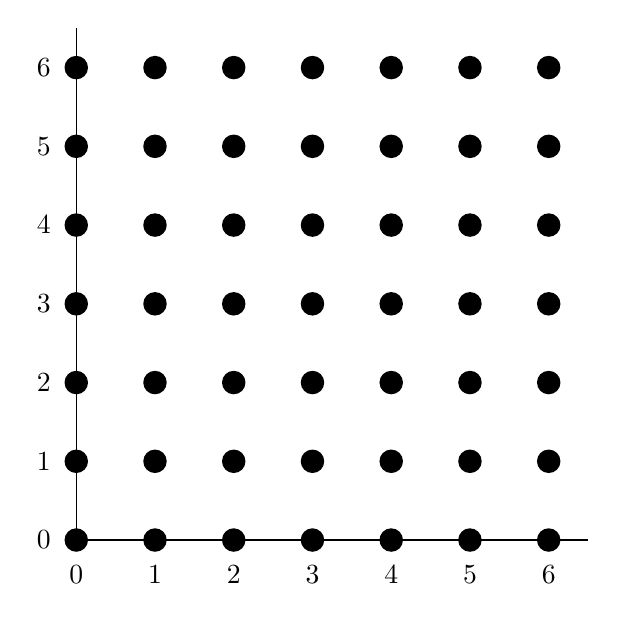
\begin{tikzpicture}[scale=1]
        \foreach \x in {0,...,6}
            {
                \foreach \y in {0,...,6}
                    {
                        \node at (\x, \y)[circle,fill,inner sep=3pt]{};
                    }
                \node[left] at (-0.2, \x){$\x$};
                \node[below] at (\x, -0.2){$\x$};
            }

        \draw (0.0, 0.0) -- (6.5, 0.0);
        \draw (0.0, 0.0) -- (0.0, 6.5);
    \end{tikzpicture}
\end{center}
这个平面上的``点阵''被称为\emph{格 (Lattice)}。一个有趣的问题是:在格中,给定任意一点,从原点 $(0, 0)$ 到该点有多少条路径?具体来说,我们将\textbf{格路径}定义为从 $(0, 0)$ 到特定点的路径,且每一步只能\emph{向右}或\emph{向上}移动。以下定义详细说明了这一概念:

\begin{definition}
    设 $(x,y) \in (\mathbb{N} \cup \{0\})^2$。到 $(x, y)$ 的\dotuline{格路径}是二维格中的一个有序格点元组,其中元组的第一个元素为 $(0, 0)$,最后一个元素为 $(x, y)$,且每个点与前一个点相比,恰好有一个坐标增加一个单位。

    更严格地说,给定 $(x, y)$,格路径是一个 $n \in \mathbb{N}$ 元组 $(P_1, P_2, \dots, P_n)$,其中每个 $P_i = (x_i, y_i)$ 是格中的一个点,且满足:
    \[\forall i \in [n - 1] \centerdot (x_{i+1}, y_{i+1}) = (x_i + 1, y_i) \lor (x_{i+1}, y_{i+1}) = (x_i, y_i + 1)\]
    同时,$(x_1, y_1) = (0, 0)$ 且 $(x_n, y_n) = (x, y)$。

    也就是说,格路径是从 $(0, 0)$ 到 $(x, y)$ 的一系列格点,其中每一步只允许向右或向上移动一个单位。
\end{definition}

\begin{example}
    考虑二维格点 $(2,4)$。如下图所示,我们展示了从原点到 $(2,4)$ 的几条格路径。

    \begin{center}
        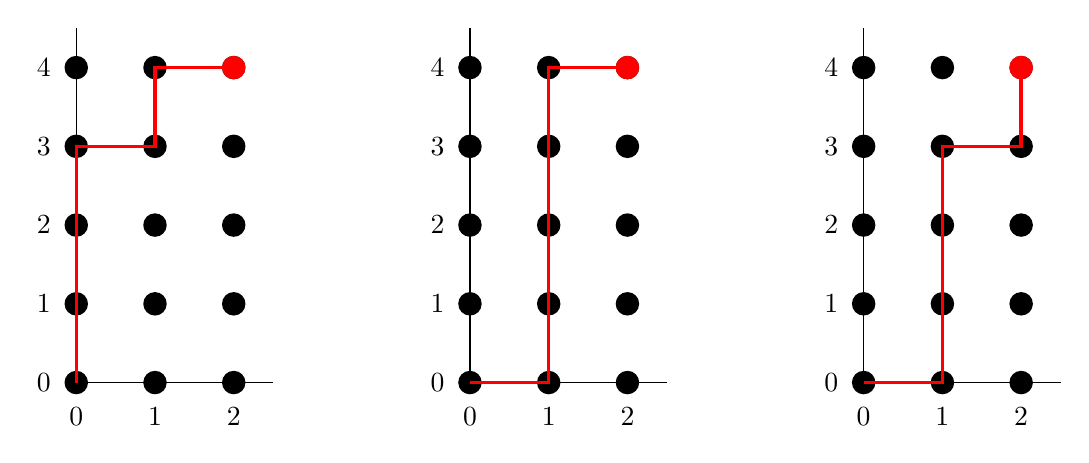
\begin{tikzpicture}[scale=1]
            \foreach \n in {0,5,10}
                {
                    \foreach \x in {0,...,2}
                        {
                            \foreach \y in {0,...,4}
                            \node at (\x+\n, \y)[circle,fill,inner sep=3pt]{};

                            \node[below] at (\x+\n, -0.2){$\x$};
                        }
                    \foreach \y in {0,...,4}
                    \node[left] at (\n-0.2, \y){$\y$};

                    \draw (\n, 0.0) -- (2.5+\n, 0.0);
                    \draw (\n, 0.0) -- (\n, 4.5);
                    \node[red] at (\n+2.0, 4.0)[circle,fill,inner sep=3pt]{};
                }
            \draw[red, very thick] (0.0, 0.0) -- (0.0, 3.0) -- (1.0, 3.0) -- (1.0, 4.0) -- (2.0, 4.0);
            \draw[red, very thick] (5.0, 0.0) -- (6.0, 0.0) -- (6.0, 4.0) -- (7.0, 4.0);
            \draw[red, very thick] (10.0, 0.0) -- (11.0, 0.0) -- (11.0, 3.0) -- (12.0, 3.0) -- (12.0, 4.0);
        \end{tikzpicture}
    \end{center}

    我们的问题是:

    \begin{quotation}
        给定 $(a,b) \in (\mathbb{N} \cup \{0\})^2$,从原点到 $(a, b)$ 有多少条\emph{不同的}格路径?
    \end{quotation}

    为了回答这个问题,我们先来看一个简单的例子,使用较小的数值以便枚举所有路径。假设我们考虑从 $(0, 0)$ 到 $(2, 2)$ 的格路径:

    \begin{center}
        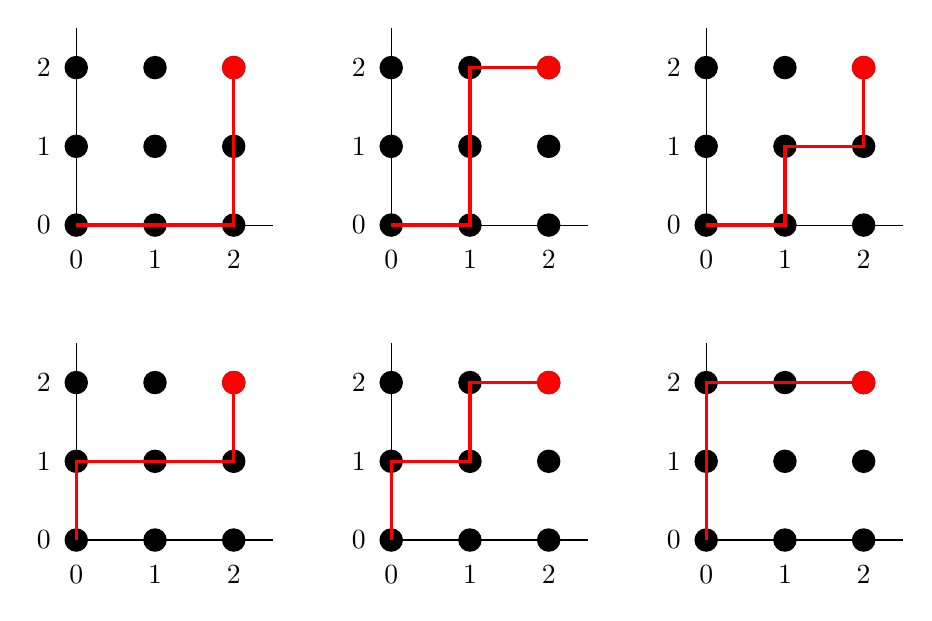
\begin{tikzpicture}[scale=1]
            \foreach \m in {0, 4}
                {
                    \foreach \n in {0, 4, 8}
                        {
                            \foreach \x in {0,...,2}
                                {
                                    \foreach \y in {0,...,2}
                                    \node at (\x+\n, \y+\m)[circle,fill,inner sep=3pt]{};

                                    \node[left] at (\n-0.2, \x+\m){$\x$};
                                    \node[below] at (\x+\n, \m-0.2){$\x$};
                                }

                            \draw (\n, \m) -- (2.5+\n, \m);
                            \draw (\n, \m) -- (\n, 2.5+\m);
                            \node[red] at (\n+2.0, \m+2.0)[circle,fill,inner sep=3pt]{};
                        }
                }
            \draw[red, very thick] (0.0, 0.0) -- (0.0, 1.0) -- (2.0, 1.0) -- (2.0, 2.0);
            \draw[red, very thick] (4.0, 0.0) -- (4.0, 1.0) -- (5.0, 1.0) -- (5.0, 2.0) -- (6.0, 2.0);
            \draw[red, very thick] (8.0, 0.0) -- (8.0, 2.0) -- (10.0, 2.0);

            \draw[red, very thick] (0.0, 4.0) -- (2.0, 4.0) -- (2.0, 6.0);
            \draw[red, very thick] (4.0, 4.0) -- (5.0, 4.0) -- (5.0, 6.0) -- (6.0, 6.0);
            \draw[red, very thick] (8.0, 4.0) -- (9.0, 4.0) -- (9.0, 5.0) -- (10.0, 5.0) -- (10.0, 6.0);
        \end{tikzpicture}
    \end{center}

    我们如何用\emph{组合的}方式来表示格路径呢?也就是说,怎样表示才能方便我们计数这些路径?回想格路径的定义:在构建路径的每一步中,每次``移动''都必须向右或向上。因此,用符号表示每次``向右''和``向上''移动是有意义的。然后,我们只需要计算有多少种由``向右''和``向上''移动组成的序列能带我们到达目标点 $(x, y)$。

    这其实很简单!平面上的点 $(x, y)$ 有什么特征呢?它位于 $(0,0)$ 的右边 $x$ 个单位、上方 $y$ 个单位。因此,无论路径如何,从 $(0,0)$ 到 $(x,y)$ 必须恰好有 $x$ 次向右移动和 $y$ 次向上移动。回顾上面到 $(2, 2)$ 的 $6$ 条格路径。想象沿着路径,从 $(0, 0)$ 开始,在每一步根据移动方向写下 $R$(右)或 $U$(上)。这样就得到了以下 $6$ 个由 $R$ 和 $U$ 组成的序列:
    \[RRUU \:,\: RUUR \:,\: RURU \:,\: URRU \:,\: URUR \:,\: UURR\]

    这些序列有什么共同特征?每个序列都有 $2$ 个 $R$ 和 $2$ 个 $U$,并且总长度为 $4$,因为从 $(0,0)$ 到 $(2,2)$ 需要 $2+2=4$ 步。这类似于一个受限的字母表/单词问题:我们希望从字母表 $\{R,U\}$ 中组成长度为 $4$ 的单词,其中 $R$ 和 $U$ 都恰好出现 $2$ 次!

    通常情况下,我们知道从 $(0,0)$ 到 $(x,y)$ 的任意格路径可以表示为一个长度为 $x+y$ 的序列,其中恰好包含 $x$ 个 $R$ 和 $y$ 个 $U$。为了确定这样的序列有多少个,我们可以分两步进行:
    \begin{enumerate}
        \item 从 $x + y$ 个空位中选择 $x$ 个填充 $R$:有 ${x+y \choose x}$ 种方式;
        \item 剩下的 $(x + y) - x = y$ 个空位填充 $U$:只有 $1$ 种确定的填充方式。
    \end{enumerate}
    因此,我们得到如下结论。

    \begin{proposition}
        对于每个 $(x,y) \in (\mathbb{N} \cup \{0\})^2$,从 $(0,0)$ 到 $(x,y)$ 恰有 ${x+y \choose x}$ 条格路径。
    \end{proposition}

    我们将在练习中探索格路径的更多应用和性质。目前,我们想强调格路径的存在及其与序列和选择之间的关系。但这里还有一个有趣的观察:为什么我们选择计算长度为 $x+y$ 的序列中恰好有 $x$ 个 $R$ 的数量?如果计算恰好有 $y$ 个 $U$ 的数量,会有什么不同吗?思考一下:每条到 $(x, y)$ 的格路径必须恰好有 $x$ 个 $R$ 和 $y$ 个 $U$,因此确保其中一个条件成立自然保证了另一个条件。于是,我们得到以下结论:

    \begin{proposition}
        对于每个 $(x,y) \in (\mathbb{N} \cup \{0\})^2$,从 $(0,0)$ 到 $(x,y)$ 恰有 ${x+y \choose y}$ 条格路径。
    \end{proposition}
    这不仅证明了如下事实
    \[{x+y \choose x} = {x+y \choose y}\]
    而且也引出了一种有用的证明策略:\textbf{两法计数}。我们确定了一组对象(从 $(0, 0)$ 到 $(x, y)$ 的格路径集合),并给出了两种\emph{不同的}计数方法。每种方法得到了该集合基数的不同表达式,因此这两个表达式必然相等。这个例子展示了两法计数的核心思想,我们将在下一节进一步探讨这一技术及其应用。
\end{example}

% !TeX root = ../../../book.tex

\subsection{习题}

\subsubsection*{温故知新}

以口头或书面的形式简要回答以下问题。这些问题全都基于你刚刚阅读的内容,所以如果忘记了具体的定义、概念或示例,可以回去重读相关部分。确保在继续学习之前能够自信地回答这些问题,这将有助于你的理解和记忆!

\begin{enumerate}[label=(\arabic*)]
    \item 如何判断一个计数方法是否\textbf{少算}了数量?又如何证明它\textbf{多算}了数量?
    \item 解释``从 $[n]$ 中选择 $k$-元组''和``字母表与单词''之间的关系。它们在本质上为何相同?
    \item 假设我们从箱子里有的 $n$ 个球中选择 $k$ 个球。为什么球是否\emph{可区分}很重要?
    \item 为什么从 $(0, 0)$ 到 ($x, y)$ 的格路径数量等于 ${x+y \choose x}$ 或 ${x+y \choose y}$?
\end{enumerate}

\subsubsection*{小试牛刀}

尝试回答以下问题。这些题目要求你实际动笔写下答案,或(对朋友/同学)口头陈述答案。目的是帮助你练习使用新的概念、定义和符号。题目都比较简单,确保能够解决这些问题将对你大有帮助!

\begin{enumerate}[label=(\arabic*)]
    \item 找出由 $5$ 张牌组成的扑克牌型中包含\textbf{两对}牌型的数量,并证明你的结论。
    \item 找出由 $5$ 张牌组成的扑克牌型中包含\textbf{葫芦}牌型的数量,并证明你的结论。
    \item 计算单词 ``\verb|COMBINATORICS|'' 的所有异序词的数量。计算单词 ``\verb|MASSACHUSETTS|''的所有异序词的数量?
    \item 考虑从 $\{1, 2, 3\}$ 中选择每个数字至少出现一次的 $4$-元组的数量。对于以下每个``证明'',通过找出一个在提出的论证中被重复计算的对象来证明它是错误的。
          \begin{enumerate}[label=(\alph*)]
              \item 在 $4$-元组的 $4$ 个位置中选一个位置放 $1$,然后选一个位置放 $2$,再选一个位置放 $3$。最后,从剩下的三个元素中选择一个放在第 $4$ 个位置。
                    \[{4 \choose 1}{3 \choose 1}{2 \choose 1}{3 \choose 1} = 72\]
              \item 从 $4$ 个位置中选择 $3$ 个位置,用元素 $1,2,3$ 填充。然后,对这 $3$ 个位置中的元素进行排列。最后,为剩下的第 $4$ 个位置选择一个数字。
                    \[{4 \choose 3} \cdot 3! \cdot 3 = 72\]
          \end{enumerate}
    \item 在这个问题中,我们将任何由英文字母组成的字符串都视为一个单词,无论它是否在字典中有实际意义。例如,\verb|ZYQFIB| 是一个长度为 $6$ 的有效单词。
          \begin{enumerate}[label=(\alph*)]
              \item 长度为 $2$ 的单词有多少个?\\
                    (用\emph{两种}方式回答该问题:一种用指数形式,另一种用两项之和。)
              \item 长度为 $7$ 的单词中,恰好包含 $3$ 个 \verb|A| 的单词有多少个?
              \item 长度为 $7$ 的单词中,最多包含 $2$ 个元音字母的单词有多少个?(注意:\verb|A, E, I, O, U| 是元音字母,\verb|Y| 不是。)
          \end{enumerate}

          考虑所有长度为 $n$ 的二进制字符串的集合 $S_n$。对于以下每个给定的性质,分别计算 $S_n$ 中有多少元素符合该性质。\\
          (注意:每个性质是独立的,不需要考虑同时满足所有性质的情况。)
          \begin{enumerate}[label=(\alph*)]
              \item 恰有 $3$ 个位置为 $0$。
              \item 最多 $3$ 个位置为 $0$。
              \item 至少 $4$ 个位置为 $0$。\\
                    (注意:用前两问的结论将 $2^n$ 写成二项式系数之和!)
              \item $0$ 比 $1$ 多。
          \end{enumerate}
    \item 设 $n \in \mathbb{N}$。共有多少条格路径可以从 $(0, 0)$ 走到 $(2n, 2n)$?又有多少条格路径会经过 $(n, n)$?
    \item 考虑下面的解释:
          \begin{quote}
              从一副标准扑克牌发出的 $6$ 张牌中,每种花色\emph{至少出现一次}的牌型数量为
              \[{13 \choose 1}{13 \choose 1}{13 \choose 1}{13 \choose 1}{48 \choose 2}\]
              因为我们先从每种花色中各选一张牌,然后再从剩下的 $48$ 张牌中选出两张。
          \end{quote}
          这个计数正确吗?如果你认为\emph{多算}了,请展示一个具体的牌型示例,并说明它是如何被重复计数的。如果你认为\emph{少算}了,请展示一个具体的牌型示例,并说明它是如何没有被计数的。
\end{enumerate}